\begin{surferPage}[216 сингуларитета]{Површи са много реалних сингуларитета}
    Kao што је поменуто, тачан максималан број сингуларитета за површи 
	седмог степена није познат.
    Знамо само да: $99\le \mu(7) \le 104$. 


    Зато и не чуди да се још мање зна за површи општег степена  $d$. 

    Оно што су Соња Бреске, Оливер Лабс и Дуко ван Стратен успели је да промене 
	конструкцију С. В. Чмутова, тако да се садашњи максималан број сингуларитета такође 
	постиже на површима са реалним сингуларитетима. 
    За сада знамо:
    \[0,41\bar{6}d^3 \lessapprox \mu(d) \lessapprox 0.44\bar{4} d^3.\]
     Из горњег се може видети симетрија конструкције и у ком је односу према максималном 
	 броју црних ћелија у распореду линија:
    \begin{center}
      \begin{tabular}{c@{\qquad}c}
        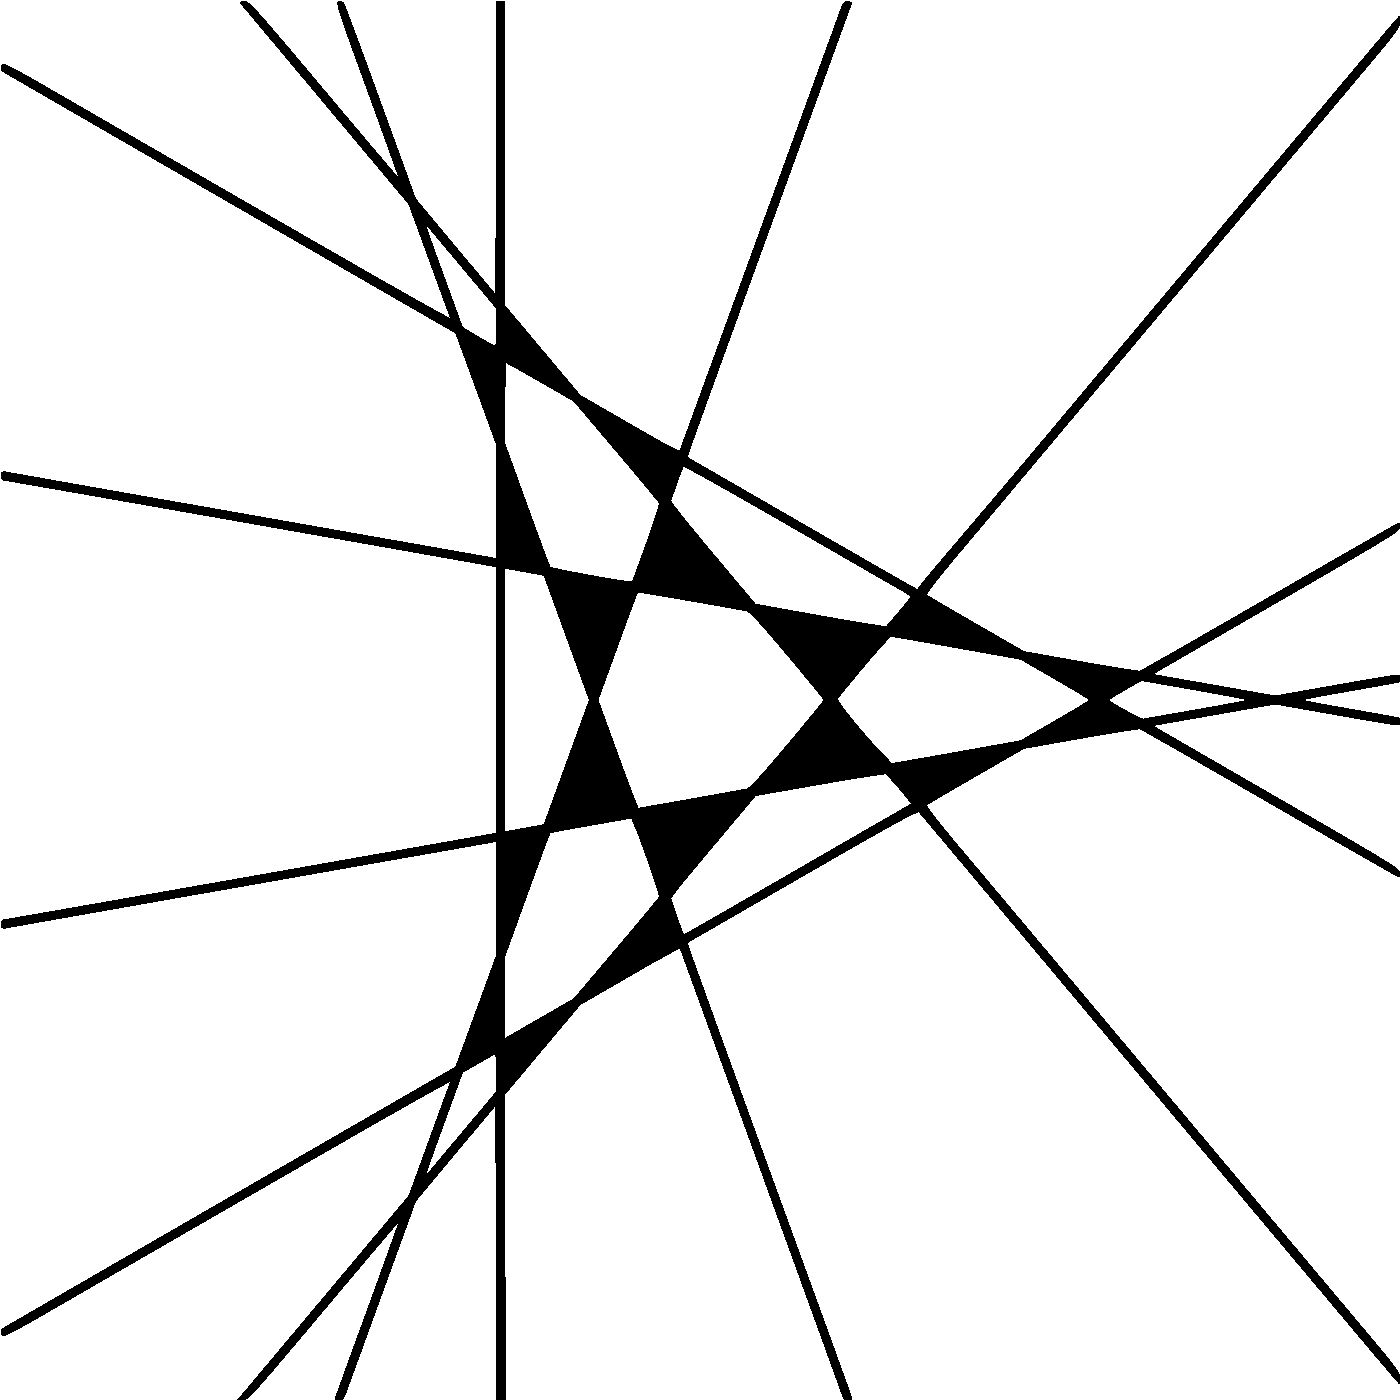
\includegraphics[height=1.5cm]{./../../common/images/vielesing.pdf}
        &
        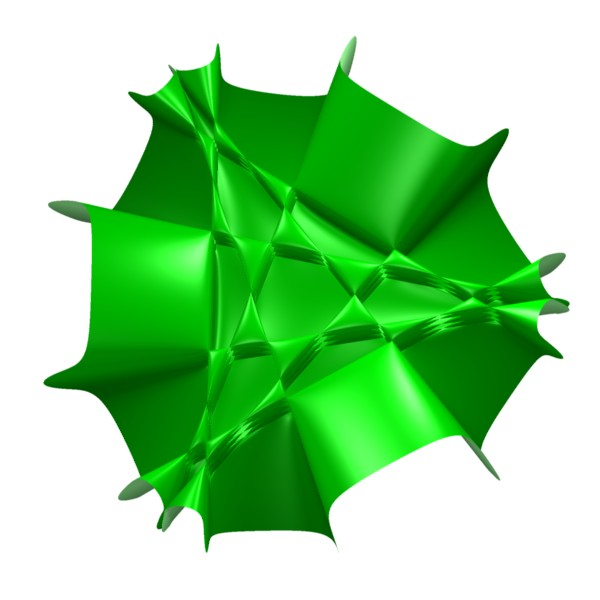
\includegraphics[height=1.5cm]{./../../common/images/p9surface_von_oben}
      \end{tabular}
    \end{center}
\end{surferPage}
